\documentclass{report}

\usepackage{Sweave}
\begin{document}
\Sconcordance{concordance:Milestone.tex:Milestone.Rnw:%
1 2 1 1 0 33 1 1 4 2 1 1 15 1 2 5 1 1 15 1 2 9 1 1 29 5 0 1 2 40 1 1 38 %
5 0 1 2 12 1 1 66 5 0 1 2 4 1 1 36 5 0 1 2 7 1 1 8 1 3 9 1 1 9 1 3 20 1}



\section{Introduction to the Problem}
Magnetic Resonance Imaging (MRI) technology, applied specifically to the brain, has given researchers an unprecedented window into the brain and enabled them to investigate how the brain's internals appear and operate. In particular when speaking about brain function, functional MRI, or fMRI, enables us to measure brain activity at different points in the brain, and across an entire time period for which the information is recorded. We can design experiments where we scan while the subject performs a certain task, and we can look at the resulting imaging sequence over time and see if brain activity patterns change while the task is performed, and for what regions does this activity change occur. 
There are inherit difficulties with fMRI data collection and analysis, and we're focused here on issues with fMRI data collection and experimental design. fMRI data collection is inherently an uncomfortable procedure for patients, (e.g. scanning children, scanning patients with conditions that make long sessions infeasible, such as ADHD, ASD). Also, issues with subject fatigue, brain conditioning to certain tasks, which may obscure unique changes we want to see in the brain. Finally, the research community is focused mroe and more on combining multiple imaging modalities, which includes structural imaging information, functional imaging information, in addition to nonimaging information, such as genetics data, other biological markers, to understand complex relationships between them. In order to do this though, an important first step is to understand each dataset more carefully, and find diverse ways to reduce the number of variables for further analysis, while maintaining maximal information, and saliency.
\subsection{What We Want To Learn}
In this project, we explore feature selection in a task based fMRI dataset for an individual subject. We want to answer the question: Can we identify a (small) subset of features in the fMRI data that can reliably predict \textit{relative} activation to a given experimental task. Results of this analysis is useful in that we can determine whether or not it is acceptable to cut down on scanning protocol, by running less runs. This information is useful for making cost saving decisions (i.e. the decision to run shorter scans), and for designing feasible scanning protocols for experiments where long runs are not feasible or difficult  (e.g. scanning children, scanning patients with conditions that make long sessions infeasible, such as ADHD, ASD).  

\subsection{Brief Overview of Functional Magnetic Resonance (fMRI) Imaging}
One major goal of gathering fMRI data is to find regions in the brain that exhibits changes in activity under various tasks.  What is measured is an indirect measurement of brain activity, called the blood oxygen level dependent signal, or BOLD signal.  In task based fMRI, we are interested in finding areas in the brain where the activity, while performing a certain task or stimulus, is significantly different from the brain's baseline activity, or different from activity due to another task. (Important to note here is that the absolute BOLD measurement in it of itself isn't useful.) Hence, when designing an fMRI experimental protocol, we need to administer a series of tasks at particular points in time.  Most common is a blocked experimental design, where each stimuli is presented for a fixed length of time, and different stimuli blocks are interleaved, together with interleaved periods for which there is no stimuli.  Preferably, for each effect to study, the corresponding condition is repeated for several trials for the duration of the scan. What is obtained by running the fMRI scan on this experiment, is a 4D (3D volume + time) dataset of BOLD intensity values at each voxel over time.
Normally, the resulting fMRI dataset is analyzed in a statistical setting using the General Linear Model. In short, you fit the GLM to the BOLD activity, where each effect is modeled as a linear predictor, and the BOLD activity is the response variable.  Using the corresponding regressors to the predictors, you apply a statistical test to determine, for each point in the image, if the given predictor significantly contributes to the response.  This is done using a t test on the regressor, with a null hypothesis of regressor = 0, or "no contribution".  Points on the image that reject the null hypothesis are considered "active", and these results are plotted over the image to create an activation map.
\subsection{Teachnical Goals}
What we would like to do is the following.  Given the activation map as a "ground truth", we want to determine how well we can predict this activation map at each image point using a simple linear model, where each time point in the BOLD signal is a descriptor. More importantly, we want to find the smallest subset of time points that gives a "similar" fit. By subset, we can mean an unstructured subset of time points, or a subset in the sense of connected subintervals of the time series. The main item of interest here is to find some insight into how much extra information is provided by repeated runs of a given effect to study. We choose to do our prediction on only one subject here for simplicity.



\section{Unpacking the Dataset}
\subsection{Description of Dataset}
The dataset we start with is raw 4D functional MR time activity information, over 3D brain image space, and time. (Pelphrey reference). We have data from 10 control subjects without any known neuropsychiatric diagnosis. The experimental design of the fMRI data is a block design. Scans are taken under the participation of 2 different visual tasks. One task consists of the subject watching a composite motion of several dots that trace out human motion, the other task consists of the subject watching a composite motion of the same dots, but instead of strategically placed to trace out human motion, are randomly scattered, hence representing motion.
\subsection{Preprocessing of the Data to get Activation Regions}
Using the knowledge of the experimental protocol, we need to first determine which regions in the brain are statistically considered "active". What we mean here is "active" when performing the biological task, \textit{relative} to the random task. That is, we want to find regions in the brain that are more active when performing the biological motion task than the random motion task. We find this by performing group-wise fMRI analysis to get a good "gold standard" of activation across the control population, following standard protocol. For each patient's fMRI data, we fit a general linear model (GLM) to the time activity curves, with the biological task and random motion task event paradigm forming the main explanatory variables (EVs), and the measured time activity as the response variable. (GLM EQUATIONS?). Before fitting this model, several preprocessing steps are applied, including motion correction across time, band pass filtering for removing linear trends and high frequency noise, and affine registration to align each subject's image to a common MNI atlas. All the analysis is performed using FSL analysis software. (REFERENCE) From all of this, we get an estimate of the regressors for the two EVs.  A two sample Z test is performed, with the test statistic BETA BIOLOGICAL - BETA RANDOM, and we threshold the Z statistic map at the desired confidence (p = .05) to get the group activation map. Now, we are ready to read in the 4D image datasets and the computed statistics into R for analysis.
\subsection{Further Data Munging}
Once all the data and the precomputed statistics are read into R, we need to tidy and organize the information into a data frame. Here, the rows, or observations, correspond to the observations at each voxel. The columns correspond to all useful the variables available across observations. These variables include the brain mask indicating valid brain issue (vs. irrelevant space/tissues such as skull), Z statistic value, cluster mask for denoting active or inactive region, and all BOLD intensities across all time points, one variable for each time point. The overall dimension of the data frame is \# voxels in image X (3 + \# time points in event paradigm). We also read in the event timing indicator series for the biological and random task, and place that into a seperate data frame. This will be useful to pick out what activity was being performed at each time point.  







\section{Exploratory Data Analysis}

We start the exploratory analysis by taking a look at the histogram of BOLD signal intensities over different subsets of the time acitivity curve, pooled over all voxels in the brain. Histograms are generated over (1) just the time points where the biological motion task is being performed, (2) just the time points where the random task is being performed, and (3) over all time points.

\begin{figure}
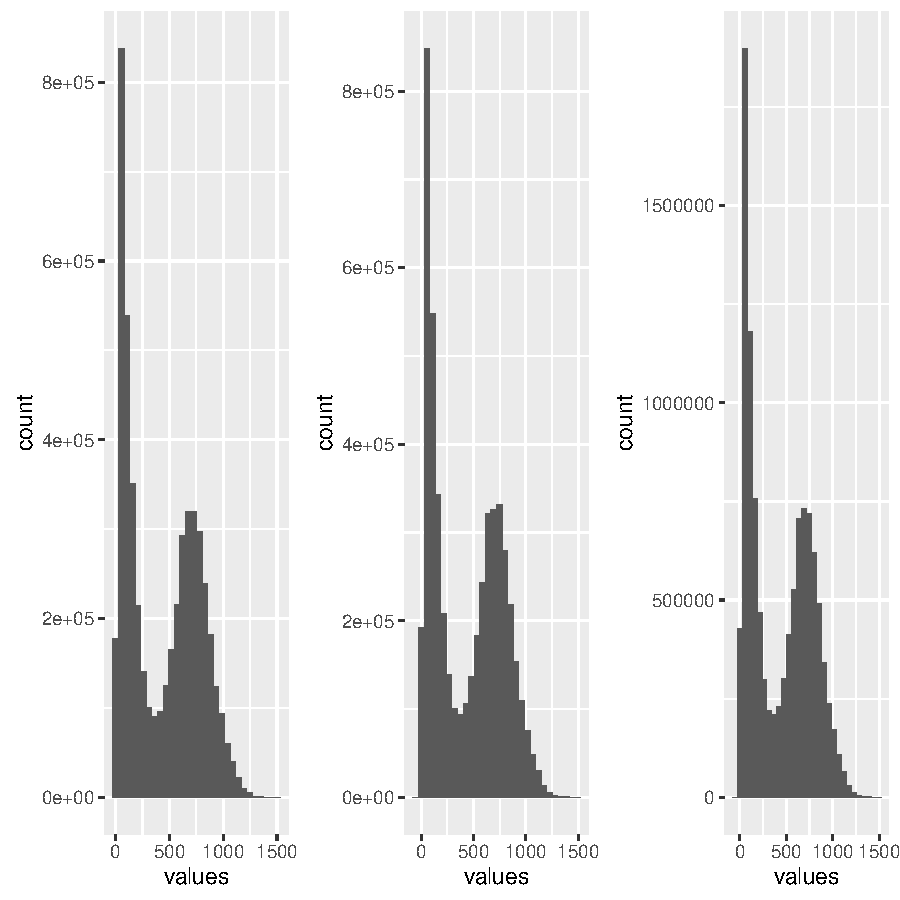
\includegraphics{Milestone-002}
\end{figure}

Upon inspection, the distribution of BOLD intensities does not vary much across the two activities. The sharp peak near 0 intensity indicates many time points exhibiting low activity. Next we look at the same distribution, but only over points deemed \textit{functionally} active by our group wise analysis.  

\begin{figure}
\caption{Same histograms as figure 1, but ONLY only voxels deemed "active" in biological task, compared to random task}
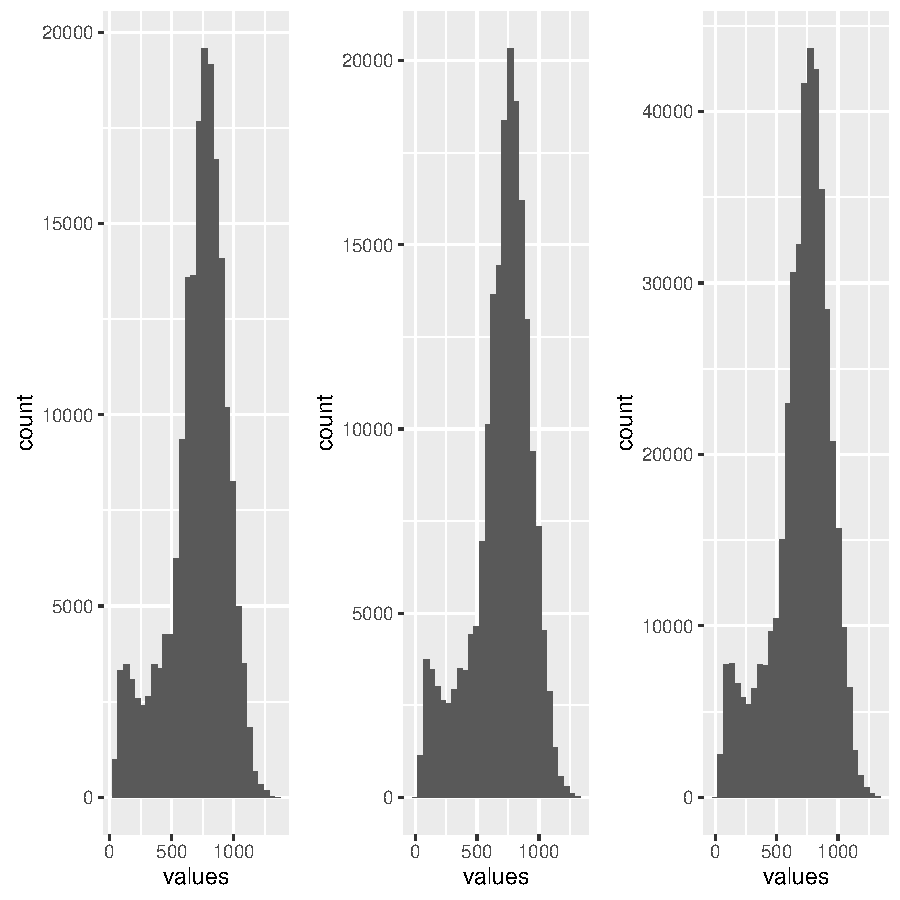
\includegraphics{Milestone-003}
\end{figure}

Here, we see a much smaller hump at low BOLD intensities. But the overall distribution still appears the same for time points under each task, so it looks like the actual response to the two tasks does not differ much across the whole brain. To further analyze, we take a look at not only the relationship between BOLD intensities and the two tasks, but also between the BOLD intensity and Z statistic  the BIOLOGICAL minus RANDOM COMPLETE THIS FORMULA, which, if we recall, is what is thresholded to give the activation map. 


\begin{figure}

\caption{Scatterplot of BOLD intensities vs. Z Statistic across combinations of biological, random task time points for active regions, and biological, random task points for inactive regions}
\label{fig:figure1}

\begin{Schunk}
\begin{Soutput}
null device 
          1 
\end{Soutput}
\end{Schunk}
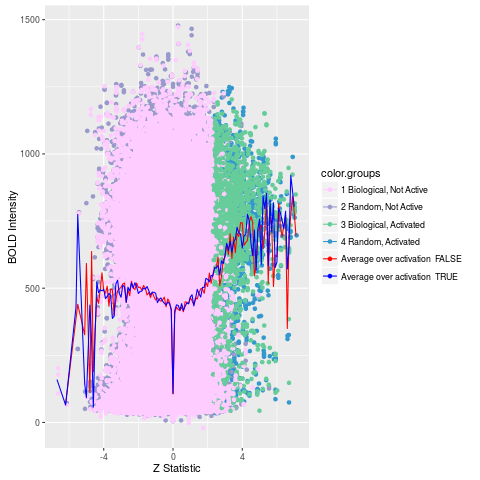
\includegraphics{fig1}

\end{figure}

%' 
%' <<echo=FALSE, fig=TRUE>>=
%' #gather all time activitry points into one column, for all masked points.
%' #introduce group factors for biological vs motion, and activation region vs. not activated
%' result <- subset(c1045.as.column, subset = BrainMask != 0) %>%
%'   gather(key = "Label", value = "Activity", 4:ncol(c1045.as.column)) %>%
%'   mutate(on.off = Label %in% names(c1045.as.column)[c(FALSE, FALSE, FALSE, paradigm$Biological)])
%' result$color.groups <- "None"
%' result$color.groups[result$ClusterMask == 0 & result$on.off == TRUE] <- "1Biological, Not Active"
%' result$color.groups[result$ClusterMask == 0 & result$on.off == FALSE] <- "2Random, Not Active"
%' result$color.groups[result$ClusterMask > 0 & result$on.off == TRUE] <- "3Biological, Activated"
%' result$color.groups[result$ClusterMask > 0 & result$on.off == FALSE] <- "4Random, Activated"
%' 
%' result$color.groups <- as.factor(result$color.groups)
%' 
%' #get just a small sample (1%) of the activity data, otherwise too many voxels
%' sampleres <- result %>% group_by(on.off) %>% sample_frac(size = .01, replace = FALSE)
%' 
%' 
%' #scatterplot of Z Statistic (biological > random) vs activity levels,
%' #for biological task ON, random taks ON
%' ggplot() +
%'   geom_point(data = sampleres, aes(x=ZStat, y=Activity, color=color.groups)) +
%'   labs(y = "BOLD Signal Level", x="Z Stat") + 
%'   geom_line(data = sampleres, aes(x=floor(ZStat*10)/10,y=floor(Activity/5)*5, color = paste("Average over activation = ",on.off)), stat="summary",   fun.y = mean) +
%'   scale_color_manual(values=c("#FFCCFF", "#9999CC", "#66CC99", "#3399CC", "Red", "Blue"))
%' @
%' 

The scatterplot confirms what we saw before with the histograms of BOLD intensities. That is, the spread of points over the biological task and random task highly overlap, across both functionally active voxels and all other voxels, and across most Z statistic values. However, the scatterplot reveals something not easily seen in the histograms, in that the spread of BOLD intensities for functionally active regions is concentrated more at higher BOLD intensity levels. Overlayed is two plots of the mean BOLD intensity at each Z statistic value, one plot averaged over functional active points, one over all other points. The mean plots confirm that on average, the BOLD signal is higher for functionally active regions. 

One important thing to note is that BOLD intensities by themselves have little use in fMRI analysis. What is more important is how the BOLD signal in each region \textit{changes} as a function of applying a task. For example, the estimated values of the regressor $\beta_{bio}$ give us an indication of how much of the BOLD time activity curve is explained by the biological task EV, or, roughly speaking, how much the BOLD activity changes are in tune with the experiment timing. So to compare a bit more "apples to apples", its useful to analyze the same scatterplot, but with the BOLD time activity curves \textit{zero centered}. The resulting centered BOLD intensity values would, in a rough sense, better represent a "change from baseline activity". 

\begin{figure}

\caption{Same histogram as figure 1, but with all time activity curves zero centered}
\label{fig:figure2}
\begin{Schunk}
\begin{Soutput}
null device 
          1 
\end{Soutput}
\end{Schunk}

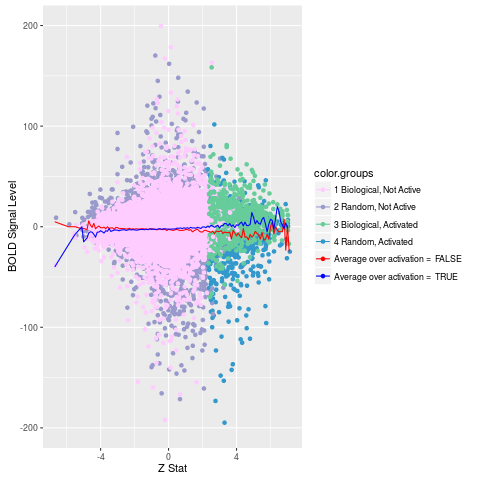
\includegraphics{fig2}
\end{figure}


From the scatterplot, we can see a slight but noticeable difference in the average BOLD intensity value curves over biological time activity points, and random time activity points. For higher Z statistic values, or \textit{active} voxels, the intensity values, on average, seem to be slightly higher when the biological motion task is being performed, which reflects the increased BOLD signal in brain regions that are involved when the task is being performed. For lower Z statistic values (i.e. inactive points), there is much less (visible) difference between the average BOLD intensities over the two tasks. This suggests that we should investigate the use of the \textit{difference} in centered BOLD time activity values over the 2 tasks, to discriminate activation regions from non active regions.

This insight inspires us to analyze differences in other summary statistics of BOLD intensity between tasks. In the following series of scatterplots, we plot just the summary statistic differences of biological minus random task, computed for each time activity curve for all voxels in the brain, against the corresponding voxel Z statistics. 

\begin{figure}

\caption{Scatterplots of differences between summary statistics of each BOLD time activity curves across biological task points and random task points}
\label{fig:figure3}
\begin{Schunk}
\begin{Soutput}
null device 
          1 
\end{Soutput}
\end{Schunk}
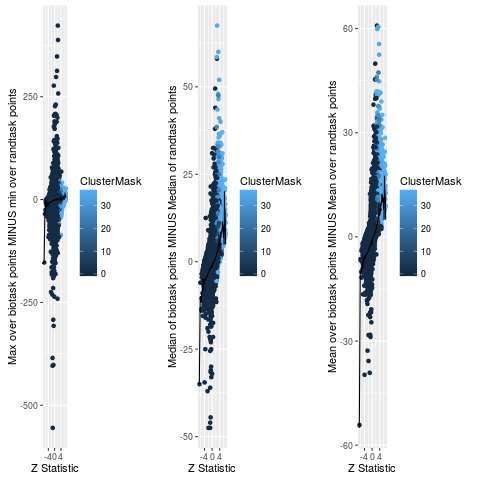
\includegraphics[width=\textwidth,keepaspectratio]{fig3}
\end{figure}

\begin{figure}
\label{fig:figure4}
\begin{Schunk}
\begin{Soutput}
null device 
          1 
\end{Soutput}
\end{Schunk}
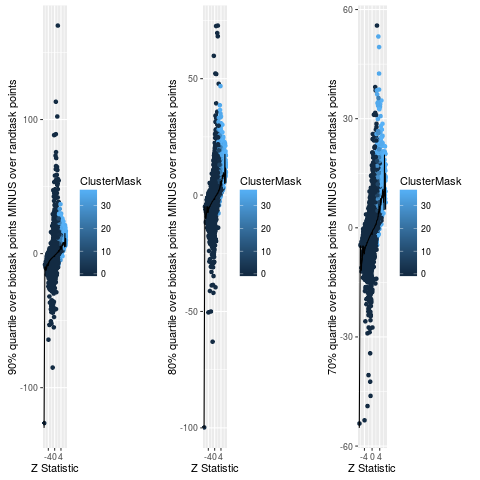
\includegraphics[width=\textwidth,keepaspectratio]{fig4}
\end{figure}

It appears that the difference of the means, as well as the difference of the 70\% quantile, gives the best spread between active and non-active points. A model can hopefully incorporate these statistics to classify functionally active regions. However, it is important to emphasize that the spread of summary statistic values overlap significantly between active regions vs inactive region points, and by themselves, do not provide a good seperation of the 2 types of regions, if the Z statistic is not available. For example, in the scatterplot of the mean difference between biological and random BOLD intensities vs Z Stat (TOP RIGHT PLOT), for the range of difference values excluding the range of values greater than 35 and less than 5, there is significant overlap of active and inactive points. A boxplot of the centered BOLD signal intensity across active and inactive points illustrates this further.

\begin{figure}
\caption{Boxplot of centered BOLD intensity across active, inactive points}
\label{fig:figure5}
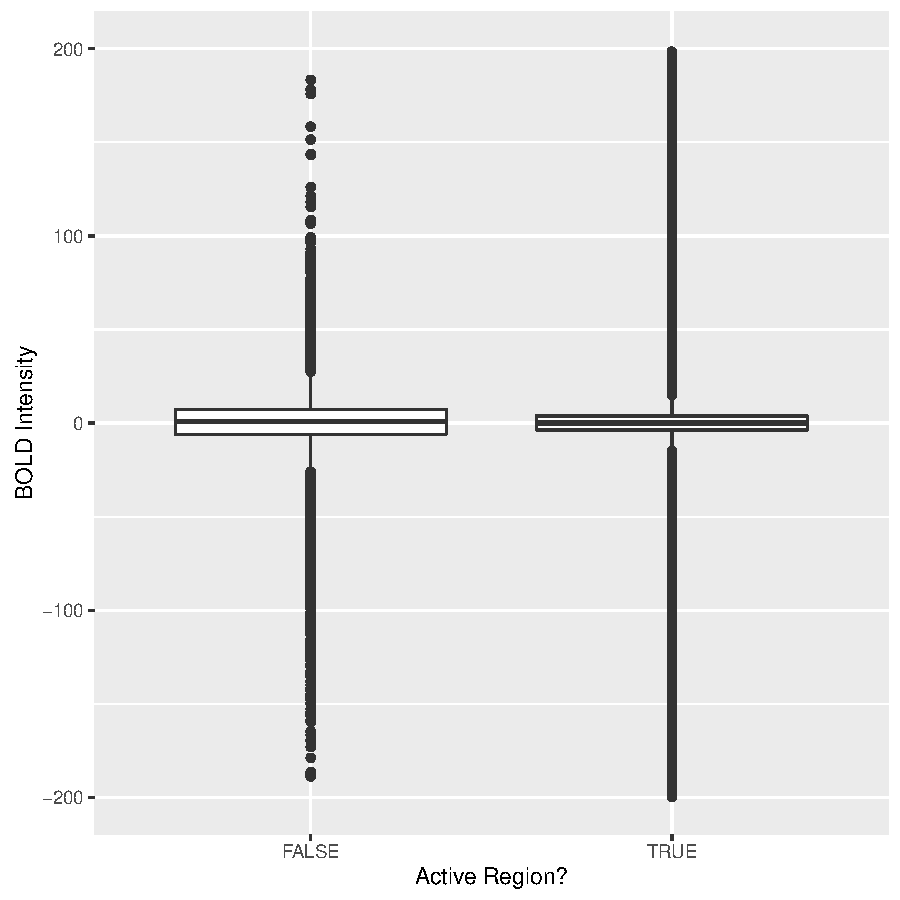
\includegraphics{Milestone-008}
\end{figure}

For both types of voxel regions, the centered BOLD signal distribution is largely concentrated about 0, with a sharp drop off indicated by the small width of the boxes. The tails are very long, notably, the tail of the distribution across active regions being longer, likely signifying time points whose activation level exhibits strong deviation from the mean signal intensity. 

One final variable to explore is Pearson's correlation coefficient of the BOLD functional time series at each voxel, to an explanatory variable time series, in particular the biological motion paradigm. Correlation is an appropriate measure of functional similarity between two time signals, since it measures the degree to which a change in one signal corresponds to a change in the same direction with the other signal. The Fisher transform is applied to the correlation coefficient values to enforce normality through variance stabalization, and the resulting values are plotted against the corresponding Z statistic.

\begin{figure}

\label{fig:figure6}
\caption{Plot of Fisher transform of correlation correlation of BOLD time series with biological task event paradigm, across Z statistic values}
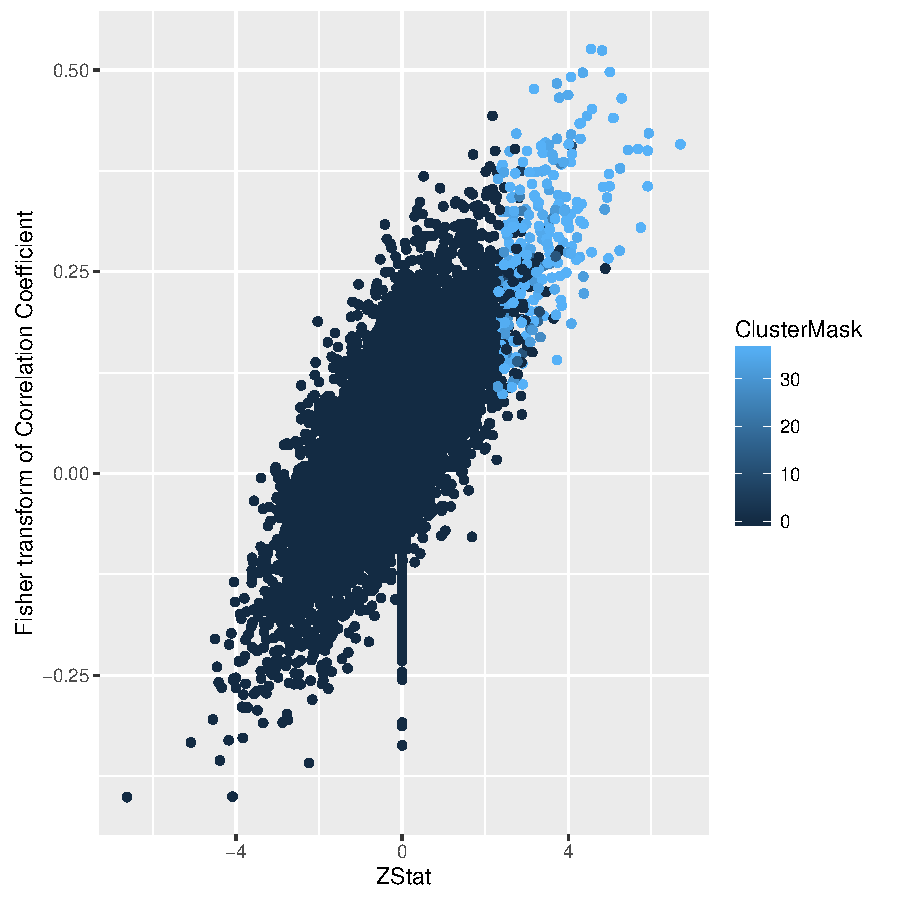
\includegraphics{Milestone-009}
\end{figure}

Here, we see a clear linear relationship between the transformed correlation coefficient and the Z stat. Further, active regions all are clustered at high correlation values.

One motivation in this project was to minimize the scan time when collecting fMRI data, effectively by reducing the number of runs of the biological and random task blocks. Hence, it is instructive to compare our exploratory data analysis on a time subset of the fMRI event paradigm. We repeat the analysis, but using only the first 2 runs of the fMRI time activity points (2 full runs of the biological task blocks interleaved with the random task blocks). The most visibly different plots are shown below.

What are its limitations i.e. what are some questions that you cannot answer with this data set?

\subsection{Main Takeaways from EDA}
The main points that we found from doing an initial data exploration is as follows:
\begin{itemize}
\item Normal BOLD activity curves, and mean centered BOLD activity curves give different information. The normal curves gives intensity values can be used to distinguish high z stat voxels vs low (or negative) values. However, on average the BOLD intensities dont vary by the task being performed, while the centered curves show some intensity differences between tasks.
\item The difference in the 75\% quartiles, and in the means of the biological task points and random task points, give most difference in BOLD intensity between active and inactive regions.
\item Correlation of BOLD activity curve to the task event paradigm has an approximately linear trend.
\item Reducing runs actually decreases spread of BOLD intensity across each z statistic. This means that a larger proportion of time activity points fall within an overlapping range of values across active and inactive points.
\item Reducing runs diminishes the linear trend between correlation coefficient and z statistic. 
\end{itemize}
The last couple bullet point is the main point of concern, because it casts some questions as to how much of a degredation in predictive power we will exhibit if we reduce the number of runs compared to using all the time series points in any kind of functional analysis of activation.
In continuing ahead with our modeling, we emphasize that we are interested in predicting activation using as smallest of a subset of time activity points, and other summary statistics. Since the group wise z statistic is a direct measure of activation, we can use the analysis from the above plots to inform our choices. Our plan is to create a model using 75\% quartile difference across biological and random task, mean difference
across the same tasks, and all BOLD time series points, and finally the correlation coefficient as predictors, and fit the model to a binary indicator of activation. The first two statistics account for extra information about differences between the tasks, and the time series points account for absolute activity.
\end{document}
